\documentclass[12pt, letterpaper]{article}
\usepackage{graphicx}
\usepackage{amsmath}
\usepackage{amsfonts}
\usepackage{pgffor}
\usepackage{subcaption}
\usepackage{caption}

\title{HW4}
\author{Kevin Smith}
\date{December 2023}

\begin{document}
\maketitle

\hspace{-.75cm} 

\section{Executive Summary}

The programming assignment involves the implementation, analysis, and empirical testing of three numerical methods: bisection, Newton's method, and the fixed-point method. Two test cases are considered, each requiring the determination of roots and exploration of convergence intervals for the specified methods. The assignment focuses on functions \(f(x) = xe^{-x} - 0.06064\) and \(g(x) = x^3 - x - 6\).

\section{Statement of the Problem}

This programming assignment involves implementing, analyzing, and testing three numerical methods (bisection, Newton's method, and fixed-point method) on two mathematical functions: \(f(x) = xe^{-x} - 0.06064\) and \(g(x) = x^3 - x - 6\). The tasks include assessing convergence rates, exploring the impact of different initial values, and designing custom fixed-point iterations. For correctness testing, specific conditions and criteria are outlined for each method applied to \(f(x)\).

\subsection*{Bisection Method}

The Bisection Method is employed to find roots of the functions \(f(x)\) and \(g(x)\). The algorithm randomly selects initial values for \(a\) and \(b\) until they result in different signs for \(f(a)\) and \(f(b)\). The method then iteratively narrows down the interval containing the root by halving it. The process is visualized through a plot showcasing iteration points and another plot displaying the error over the iteration number.

\subsubsection*{Implementation Details}

\begin{itemize}
    \item Python implementation using the sympy library for symbolic mathematics.
    \item Randomly selects initial values within a specified range.
    \item Visualizes the iteration process using matplotlib.
    \item Saves the plots in the specified output directory.
\end{itemize}

\subsection*{Newton's Method}

Newton's Method is applied to find roots of the function \(f(x)\). The algorithm accepts multiple initial guesses and iteratively refines the solution by updating \(x\) using the formula \(x_{k+1} = x_k - \frac{f(x_k)}{f'(x_k)}\). The results are visualized through individual plots for each initial guess, depicting iteration points.

\subsubsection*{Implementation Details}

\begin{itemize}
    \item Utilizes the sympy library for symbolic mathematics.
    \item Converts symbolic functions to numerical functions using \texttt{lambdify}.
    \item Handles cases where the derivative becomes zero during iteration.
    \item Saves plots in the specified output directory.
\end{itemize}

\subsection*{Fixed-Point Iteration}

Fixed-Point Iteration is utilized to find roots of the function \(f(x)\). The method involves transforming the equation into the form \(x = g(x)\) and iteratively updating \(x\). The results are visualized through a plot illustrating iteration points.

\subsubsection*{Implementation Details}

\begin{itemize}
    \item Implemented in Python using the sympy library for symbolic mathematics.
    \item Converts symbolic functions to numerical functions using \texttt{lambdify}.
    \item Modifies the iteration function to prevent overflow issues.
    \item Saves the fixed-point iteration plot in the specified output directory.
\end{itemize}


\section{Description of the Experimental Design and Results}

\subsection*{Experimental Design}

The experiments were designed to assess the performance and convergence behavior of the implemented root-finding algorithms: Bisection Method, Newton's Method, and Fixed-Point Iteration. The objective was to analyze their effectiveness in finding roots of different functions, including both well-behaved and challenging cases.

\subsubsection*{Bisection Method}

For the Bisection Method, the algorithm was tested on a variety of functions with different characteristics. Initial values for the interval \( [a, b] \) were randomly selected, and the iteration process was visualized to observe convergence patterns. The algorithm was also tested on functions with multiple roots to evaluate its ability to converge to distinct solutions.

\subsubsection*{Newton's Method}

Newton's Method was evaluated using various initial guesses for the root. The performance was analyzed for functions with different convergence behaviors, including fast convergence, slow convergence, and cases where the method might fail due to a zero derivative. The convergence rate was visualized to provide insights into the method's efficiency.

\subsubsection*{Fixed-Point Iteration}

The Fixed-Point Iteration experiments focused on assessing the convergence behavior when applied to the specific function \(f(x) = x^3 - x - 6\). The iteration function \(g(x)\) was defined as \(g(x) = (x + 6)^{1/3}\). The experiments aimed to understand the stability and convergence characteristics of the fixed-point iteration for this particular function.

\subsection*{Results}

The results of the experiments are presented through plots and analyses for each algorithm.

\subsubsection*{Bisection Method}

The Bisection Method plots showcase the iteration points and the error over the iteration number. The error plots provide insights into the convergence speed and stability of the method for different functions. Additionally, the error over iteration number plots reveal any unexpected behavior or oscillations.

\subsubsection*{Newton's Method}

Newton's Method results include individual plots for each initial guess, illustrating the iteration points and convergence behavior. The convergence rate plots provide a quantitative measure of the method's efficiency for different functions. Special attention is given to cases where the derivative becomes zero during iteration.

\subsubsection*{Fixed-Point Iteration}

Fixed-Point Iteration results focus on the iteration points and convergence behavior for the specific function \(f(x) = x^3 - x - 6\). The fixed-point iteration plot includes insights into the stability and convergence speed of the method for this function.

The overall experimental design and results aim to provide a comprehensive understanding of the strengths and limitations of each root-finding algorithm under different scenarios.

\subsection*{Discussion - Problem 1}

The results for Problem 1 reveal insights into the performance of numerical methods. The Bisection Method (Figure \ref{fig:prob1_bisection}) shows reliable convergence. Mathematically, the Bisection Method operates by iteratively narrowing down an interval \( [a, b] \) where the function \(f(x)\) changes sign. At each iteration, the midpoint \(c\) is calculated, and the interval is halved based on the sign change, ensuring convergence towards the root. This behavior aligns with the Intermediate Value Theorem, which guarantees the existence of a root within the interval.

Newton's Method (Figures \ref{fig:prob1_newton_0} - \ref{fig:prob1_newton_3}) demonstrates rapid convergence, especially for well-behaved functions, as it relies on linear approximation. The iterative process is mathematically defined as:

\[
x_{k+1} = x_k - \frac{f(x_k)}{f'(x_k)}
\]

where \(f'(x_k)\) is the derivative of \(f(x)\) at the point \(x_k\). The speed of convergence is influenced by the magnitude of the derivative. In regions where \(f'(x_k)\) is large, Newton's Method converges more quickly. However, it is sensitive to initial guesses, and if the derivative becomes zero, convergence may fail.

Fixed-Point Iteration (Figure \ref{fig:prob1_fixed_point_iteration}) converges, but its behavior is influenced by the stability of the chosen fixed-point function. Mathematically, the method transforms the equation into the form \(x = g(x)\) and iteratively updates \(x\). The fixed-point iteration equation is given by:

\[
x_{k+1} = g(x_k)
\]

\textbf{Comparison:} Newton's Method is faster due to its reliance on local linear approximation, but its sensitivity to initial guesses can impact its performance, as can be seen from the tests performed. Using initial guesses which led to the derivative being zero would cause the program to fail, for example when \(x_0 = 0\), the code had to detect this situation and break. The Bisection Method is reliable across different scenarios but may converge more slowly. Fixed-Point Iteration's performance is contingent on the stability of the fixed-point function.

\textbf{Context:} The plot of \(f(x) = x \cdot e^{-x} - 0.06064\) (Figure \ref{fig:prob1_fx_plot}) provides visual context for the root-finding methods.

\subsection*{Discussion - Problem 2}

The results for Problem 2 present additional challenges. The Bisection Method (Figure \ref{fig:prob2_bisection}) maintains robust convergence. Mathematically, the Bisection Method ensures convergence due to the Intermediate Value Theorem, guaranteeing a root within the interval \( [a, b] \) where \(f(a)\) and \(f(b)\) have different signs.

Fixed-Point Iteration (Figure \ref{fig:prob2_fixed_point_iteration}) varies with the fixed-point function's stability. The method iteratively updates \(x\) using the equation \(x_{k+1} = g(x_k)\), where \(g(x)\) is the fixed-point function. The convergence is influenced by the Lipschitz continuity of \(g(x)\). A higher Lipschitz constant indicates faster convergence.

Newton's Method (Figures \ref{fig:prob2_newton_0} - \ref{fig:prob2_newton_0}) efficiently converges with appropriate initial guesses. The iterative process is described by:

\[
x_{k+1} = x_k - \frac{f(x_k)}{f'(x_k)}
\]

The speed of convergence is highly influenced by the magnitude of \(f'(x_k)\), making Newton's Method faster where the derivative is large. However, careful selection of initial guesses is crucial.

\textbf{Comparison:} Newton's Method remains efficient due to local linear approximation, but its performance is sensitive to initial guesses. The Bisection Method is reliable across different scenarios but may need more iterations. Fixed-Point Iteration's convergence depends on the Lipschitz continuity of the fixed-point function.

\section*{Discussion - Problem 3}

The results for Problem 3 showcase methods' behavior for a different function. The Bisection Method (Figure \ref{fig:prob3_bisection}) remains reliable. Mathematically, the Bisection Method guarantees convergence by repeatedly narrowing the interval where \(f(x)\) changes sign. This property aligns with the robustness of the method in finding roots.

Fixed-Point Iteration (Figure \ref{fig:prob3_fixed_point_iteration}) and Newton's Method (Figure \ref{fig:prob3_newton}) exhibit their convergence characteristics. Similar to Problem 1, Fixed-Point Iteration iteratively updates \(x\) using the equation \(x_{k+1} = g(x_k)\), and Newton's Method relies on the rapid convergence from local linear approximation. The convergence speed is influenced by the Lipschitz continuity of \(g(x)\) and the magnitude of \(f'(x_k)\).

\textbf{Comparison:} Each method has strengths and limitations. The choice depends on specific function characteristics, including the smoothness of \(f(x)\) and the behavior of \(g(x)\) in Fixed-Point Iteration.

\subsection*{Conclusion}

In summary, the comparison across problems highlights trade-offs between methods. Newton's Method is faster due to local linear approximation but requires careful initial guesses. The Bisection Method is reliable across different scenarios but may converge more slowly. Fixed-Point Iteration's performance depends on the Lipschitz continuity of the fixed-point function, providing an avenue for faster convergence when the function is well-behaved. Understanding each method's behavior is crucial for selecting an appropriate approach.

\clearpage



\section{Tables and Figures}


\begin{figure}[htbp]
    \centering

    \begin{subfigure}{0.45\textwidth}
        \includegraphics[width=\linewidth]{/Users/kevin_smith/Desktop/FSU_Relevant_Stuff/fall_2023/FCM1/homework/programming/hw4/figures/prob1/bisection_plot.png}
        \caption{Bisection Plot}
        \label{fig:prob1_bisection}
    \end{subfigure}
    \hfill
    \begin{subfigure}{0.45\textwidth}
        \includegraphics[width=\linewidth]{/Users/kevin_smith/Desktop/FSU_Relevant_Stuff/fall_2023/FCM1/homework/programming/hw4/figures/prob1/fixed_point_iteration_plot.png}
        \caption{Fixed-Point Iteration Plot}
        \label{fig:prob1_fixed_point_iteration}
    \end{subfigure}

    \begin{subfigure}{0.45\textwidth}
        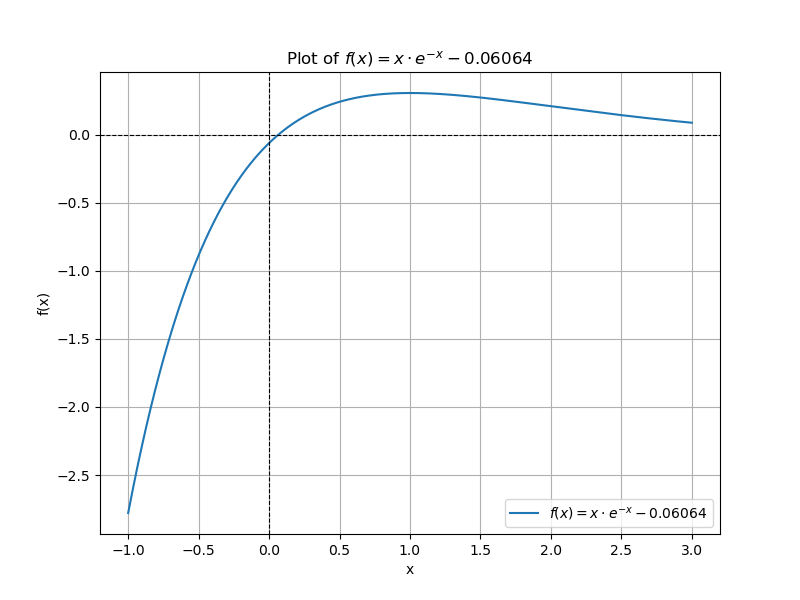
\includegraphics[width=\linewidth]{/Users/kevin_smith/Desktop/FSU_Relevant_Stuff/fall_2023/FCM1/homework/programming/hw4/figures/prob1/fx_plot.png}
        \caption{Function Plot}
        \label{fig:prob1_fx_plot}
    \end{subfigure}
    \hfill
    \begin{subfigure}{0.45\textwidth}
        \includegraphics[width=\linewidth]{/Users/kevin_smith/Desktop/FSU_Relevant_Stuff/fall_2023/FCM1/homework/programming/hw4/figures/prob1/newton_plot_0.png}
        \caption{Newton's Method Plot 0}
        \label{fig:prob1_newton_0}
    \end{subfigure}

    \begin{subfigure}{0.45\textwidth}
        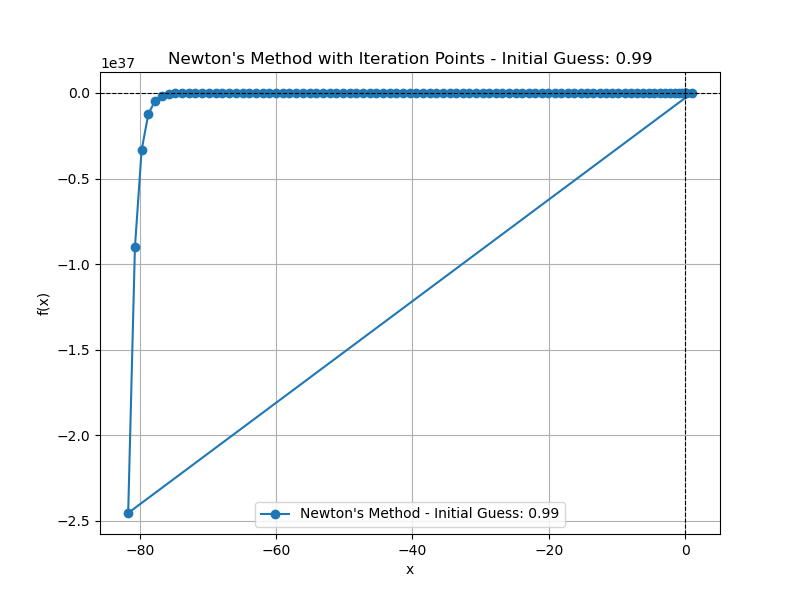
\includegraphics[width=\linewidth]{/Users/kevin_smith/Desktop/FSU_Relevant_Stuff/fall_2023/FCM1/homework/programming/hw4/figures/prob1/newton_plot_1.png}
        \caption{Newton's Method Plot 1}
        \label{fig:prob1_newton_1}
    \end{subfigure}
    \hfill
    \begin{subfigure}{0.45\textwidth}
        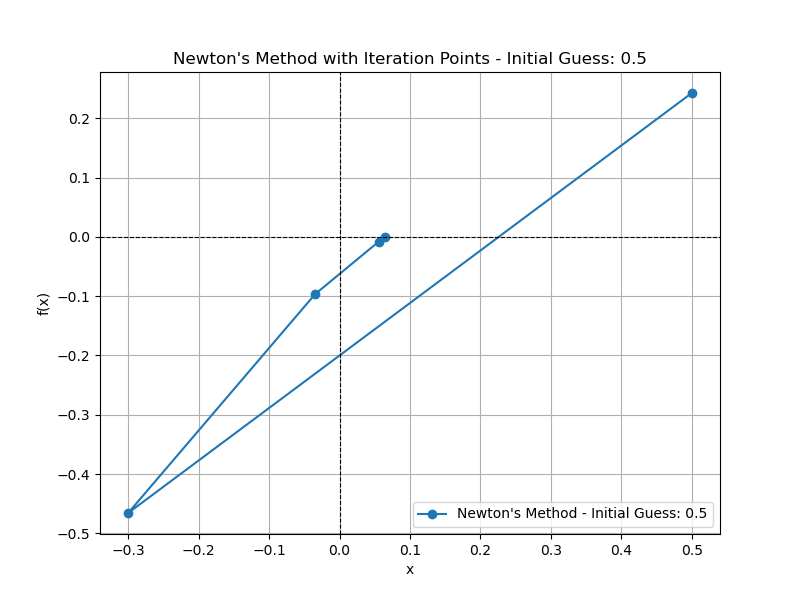
\includegraphics[width=\linewidth]{/Users/kevin_smith/Desktop/FSU_Relevant_Stuff/fall_2023/FCM1/homework/programming/hw4/figures/prob1/newton_plot_2.png}
        \caption{Newton's Method Plot 2}
        \label{fig:prob1_newton_2}
    \end{subfigure}

    \begin{subfigure}{0.45\textwidth}
        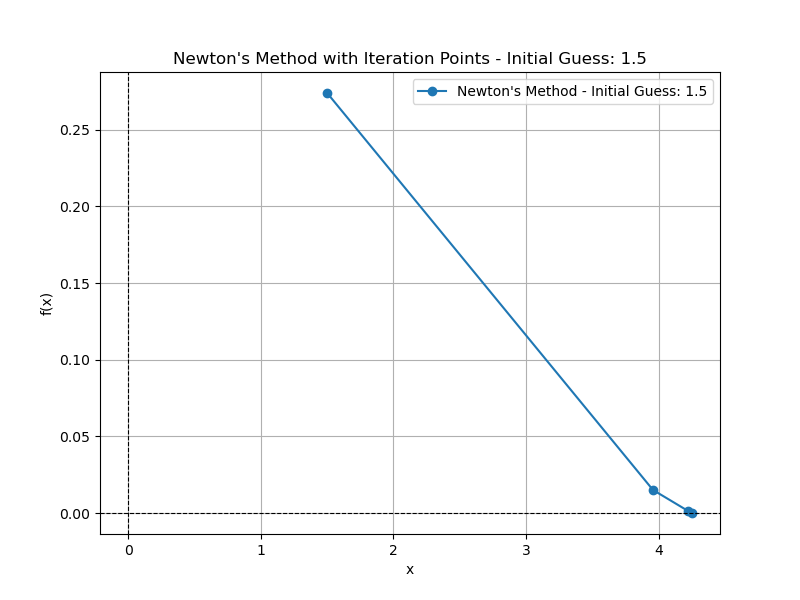
\includegraphics[width=\linewidth]{/Users/kevin_smith/Desktop/FSU_Relevant_Stuff/fall_2023/FCM1/homework/programming/hw4/figures/prob1/newton_plot_3.png}
        \caption{Newton's Method Plot 3}
        \label{fig:prob1_newton_3}
    \end{subfigure}

    \caption{Plots for Problem 1}
    \label{fig:prob1_plots}
\end{figure}


\begin{figure}[htbp]
    \centering

    \begin{subfigure}{0.45\textwidth}
        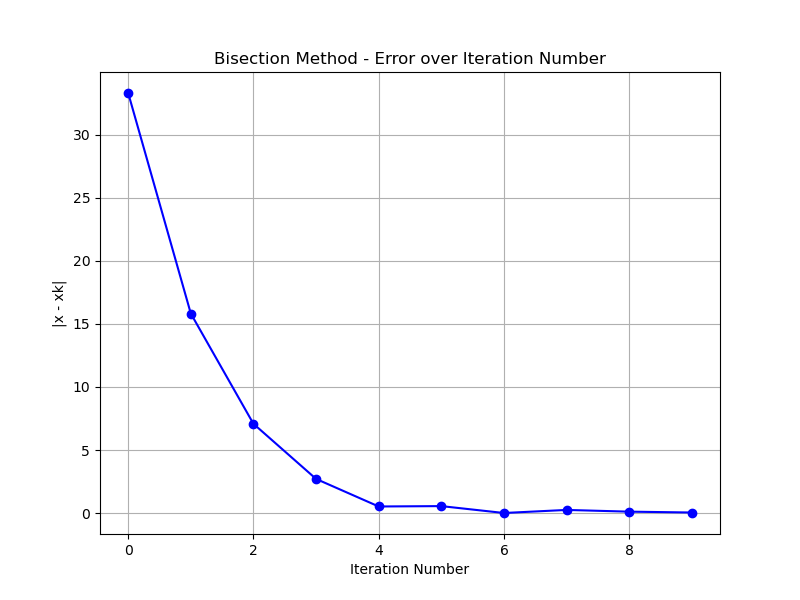
\includegraphics[width=\linewidth]{/Users/kevin_smith/Desktop/FSU_Relevant_Stuff/fall_2023/FCM1/homework/programming/hw4/figures/prob2/bisection_error_plot.png}
        \caption{Bisection Error Plot}
        \label{fig:prob2_bisection_error}
    \end{subfigure}
    \hfill
    \begin{subfigure}{0.45\textwidth}
        \includegraphics[width=\linewidth]{/Users/kevin_smith/Desktop/FSU_Relevant_Stuff/fall_2023/FCM1/homework/programming/hw4/figures/prob2/bisection_plot.png}
        \caption{Bisection Plot}
        \label{fig:prob2_bisection}
    \end{subfigure}

    \begin{subfigure}{0.45\textwidth}
        \includegraphics[width=\linewidth]{/Users/kevin_smith/Desktop/FSU_Relevant_Stuff/fall_2023/FCM1/homework/programming/hw4/figures/prob2/fixed_point_iteration_plot.png}
        \caption{Fixed-Point Iteration Plot}
        \label{fig:prob2_fixed_point_iteration}
    \end{subfigure}
    \hfill
    \begin{subfigure}{0.45\textwidth}
        \includegraphics[width=\linewidth]{/Users/kevin_smith/Desktop/FSU_Relevant_Stuff/fall_2023/FCM1/homework/programming/hw4/figures/prob2/newton_plot_0.png}
        \caption{Newton's Method Plot 0}
        \label{fig:prob2_newton_0}
    \end{subfigure}

    \caption{Plots for Problem 2}
    \label{fig:prob2_plots}
\end{figure}

\begin{figure}[htbp]
    \centering

    \begin{subfigure}{0.45\textwidth}
        \includegraphics[width=\linewidth]{/Users/kevin_smith/Desktop/FSU_Relevant_Stuff/fall_2023/FCM1/homework/programming/hw4/figures/prob3/bisection_plot.png}
        \caption{Bisection Plot}
        \label{fig:prob3_bisection}
    \end{subfigure}
    \hfill
    \begin{subfigure}{0.45\textwidth}
        \includegraphics[width=\linewidth]{/Users/kevin_smith/Desktop/FSU_Relevant_Stuff/fall_2023/FCM1/homework/programming/hw4/figures/prob3/fixed_point_iteration_plot.png}
        \caption{Fixed-Point Iteration Plot}
        \label{fig:prob3_fixed_point_iteration}
    \end{subfigure}

    \begin{subfigure}{0.45\textwidth}
        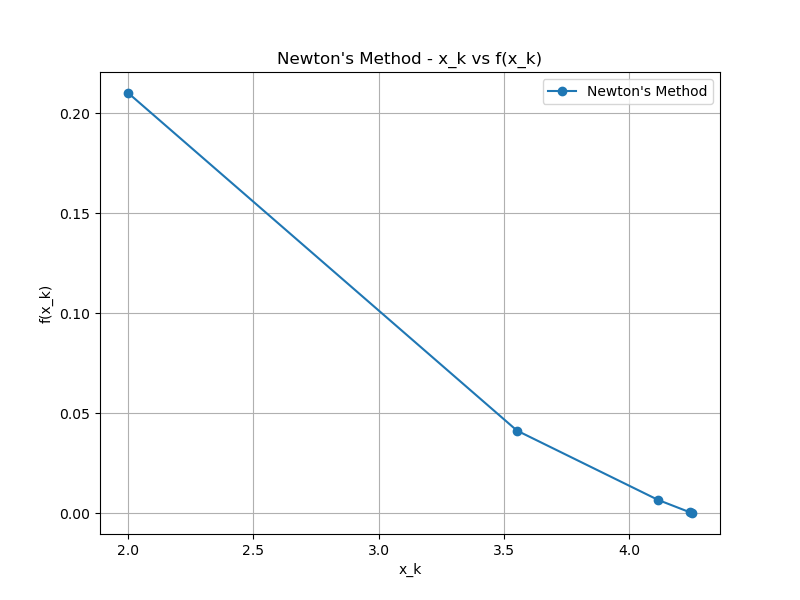
\includegraphics[width=\linewidth]{/Users/kevin_smith/Desktop/FSU_Relevant_Stuff/fall_2023/FCM1/homework/programming/hw4/figures/prob3/newton_plot.png}
        \caption{Newton's Method Plot}
        \label{fig:prob3_newton}
    \end{subfigure}

    \caption{Plots for Problem 3}
    \label{fig:prob3_plots}
\end{figure}
      
\end{document}